\documentclass[12pt,letterpaper]{article}
\usepackage{amsmath}
\usepackage{amssymb}
\usepackage{amsthm}

\usepackage{algorithm}
\usepackage{algpseudocode}
\usepackage{xcolor}
\usepackage{tikz}
\usepackage{float}

\newcommand*{\bigo}{\mathcal{O}}
\newcommand*{\R}{\mathbb{R}}
\newtheorem{theorem}{theorem}[section]
\newtheorem{definition}[theorem]{Definition}
\newtheorem{lemma}[theorem]{Lemma}
\newtheorem{corollary}[theorem]{Corollary}
\newtheorem{observation}[theorem]{Observation}



\title{A Convex Hull for Airplane Refueling Problem(subject to change)}
\author{Zixuan Fan}

\begin{document}

\maketitle

\section{Motivation}
This project aims to a description of the convex hull for the linear programming description of the 
airplane refueling problem. The problem lies in the field of mathematical optimization, 
which is an interdisciplinary branch of mathematics and computer science. In addition, 
an aspect of theorectial computer science is also involved: the computational complexity of the problem 
is a foundamental goal for the problem, and is worthing studying in the project. The project suits me well for two reasons.
\begin{itemize}
    \item My application area in bachelor's study was mathematics, where I took the course Einführung in die Optimierung. This course provides proper background knowledges for the project. 
    \item My main interest in master's study is theorectical computer science. The project is a good opportunity for me to combine my interest in mathematics and computer science.
\end{itemize}

\section{Project Description}
\subsection{Theoretical Foundations}
A natural language description of air plane refueling problem by \cite{puzzle}
\begin{quotation}
    Given a sequence of airplanes filled with fuel. Suppose they can refill each other while flying.
    What is the longest distance/flying time the last plane can reach?
\end{quotation}
A formal definition by \cite{woeginger2010scheduling} is based on the following assumptions
\begin{itemize}
    \item The airplanes are flying in a straight line.
    \item All airplanes consume the fuel of only one airplane simultaneously
    \item Whenver an airplane runs out of fuel, it lands immediately.
    \item We use flying time instead of distance for the objective function
\end{itemize}
The problem is formulated as follows
\begin{definition}
    Given $n$ planes, each with its capacity $w_j$ and fuel consumption rate $p_j$. What is the maximal flying time the last plane can reach?
\end{definition}
A reduction to scheduling problem was found. Let $C_j$ denote the completion time of job $j$, i.e. the flying time of the plane $i$.
The optimization goal is 
\begin{align*}
    \min -\sum_{j=0}^n w_j / C_j
\end{align*}
Many researchers focus on the precedence of the problem for an efficient algorithm \cite{li2019fast} \cite{vasquez2015airplane},
In this project, I will examine the problem from another aspect: convex hull of the schedule vectors, $(1/C_1, ..., 1/C_n)$.

\subsection{Practical Goals}
Aside from the theoretical aspect, the convex hull needs to be actually computed given an instance of the problem. 
This requires to take advantage of the existing software, e.g. Polymake. Polymake is a software for research in polyhedral geometry.
It can help to compute the polytopes and polyhedra, which potentially makes up the desired convex hull in this project. 
The practical goal will be exploiting the software to compute the convex hull for a large scale of instances. 
This can be separated into two subgoals:
\begin{itemize}
    \item Generate the instances of the problem both at random and using some extreme edge cases. Build up a framework such that one 
    may call the software to compute the convex hull for the instances. The software should not be limited to Polymake. 
    \item Exploiting some unsupervised learning techniques to analyze the data. Ideally, this will be helpful to find some property 
    that is not obvious from the data.
\end{itemize}

\section{Course to visit from another subject}
The course I would like to visit is Combinatorial Optimization(MA4502) offered by the department of Mathematics at School of CIT.
This course deals with application of linear programming in many combinatorial problems such as netflows, matching etc. 
In addition, it also studies approximation of NP-hard problems via linear programming. Through learning of the course, 
I believe I will obtain more insights into handling of combinatorial problems, and ideally be able to work on the project. 

\section{Timetable and Milestones}
The desired duration of this project is five months. The project can be divided into three phases.
\begin{enumerate}
    \item The first phase involves reading literatures and doing small experiments. The goal is building up a framework which enables larger experiments in the second phase. 
    \item The second phase is the main practical part of the project. It requires to call and run the scientific software that help to compute the convex hull on a large scale. 
    In addition, my task would be examine and determine the potential geometrical property of the convex hull. Some machine learning techniques may be employed in this phase 
    for the analysis of the data.
    \item If certain property is detected in the second phase. The third phase will be focusing on explore the exact property and ideally give a proof sketch for the property. 
    If the second phase fails to detect any property, further data analyses will be performed in this phase. 
\end{enumerate}
A visualization and summary of timetable and milestones can be found in the following flow graph. 
\begin{figure}[H]
    \centering 
    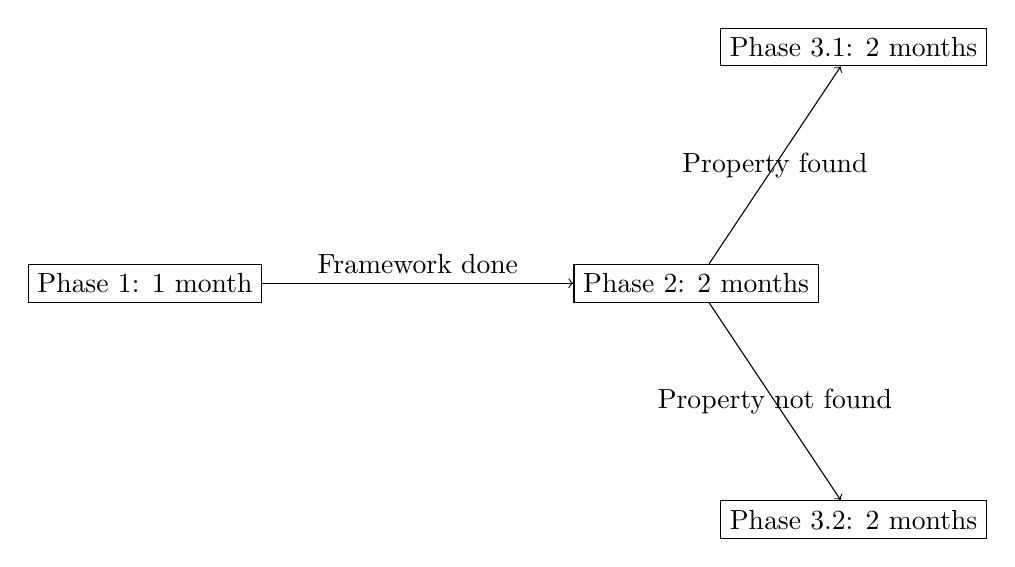
\begin{tikzpicture}
        \node[draw] (1) at (-2, 0) {Phase 1: 1 month};
        \node[draw] (2) at (5, 0) {Phase 2: 2 months};
        \node[draw] (3) at (7, 3) {Phase 3.1: 2 months};
        \node[draw] (4) at (7, -3) {Phase 3.2: 2 months};
        \draw[->] (1) -- node[above] {Framework done} (2) ;
        \draw[->] (2) -- node {Property found} (3) ;
        \draw[->] (2) -- node {Property not found} (4);
    \end{tikzpicture}
\end{figure}
The project will start as of the start of May. 
If the registration is delayed, I would like to delay the timetable for each phase accordingly.



\bibliographystyle{plain}
\bibliography{citations}
\end{document}